\documentclass{article}

% ======================== %
% ===== Use Packages ===== %
% ======================== %

\usepackage[a4paper]{geometry}
\usepackage{lmodern}
\usepackage[OT1]{fontenc}
\usepackage{varwidth}
\usepackage{amsthm} 
\usepackage{amssymb}
\usepackage{amsmath}
\usepackage{listing}
\usepackage{graphicx}
\usepackage{tikz}
\usepackage{calc}
\usepackage{mathrsfs}


% ======================== %
% ===== TiKZ Goodies ===== %
% ======================== %

\usetikzlibrary{arrows,positioning,intersections,calc}
\usetikzlibrary{decorations.markings}
\usetikzlibrary{arrows.meta}

% for morphisms in free or commutative diagrams
\tikzset{
  morphism/.style=-{ To[length=1.52mm, width=1.5mm] }
} 

\newtheorem{question}{Question}

\begin{document}
\section*{CTfP Challenges --- Chapter 14: Representable Functors}
    \begin{question}
        Show that the hom-functors map identity morphisms in $\mathscr{C}$ to corresponding identity
        functions in $\mathbf{Set}$
    \end{question}
    Consider objects $X,Y,Z$ along with morphisms $X \xrightarrow{\ f\ } Z$ and $Y \xrightarrow{\ 
    h_0,\ h_1,\ \dots\ h_n\ } X$. By functoriality, we know that the Hom functor $\mathscr{C}(Y,-)$ 
    maps the morphism $f$ to some function from the homset $\mathscr{C}(Y,X)$ to the homset 
    $\mathscr{C}(Y,Z)$. Specifically, this function will send each $h_n \in \mathscr{C}(Y,X)$ to $f 
    \circ h_n \in \mathscr{C}(Y,Z)$. We can see this more clearly with a diagram:

    \begin{center}
        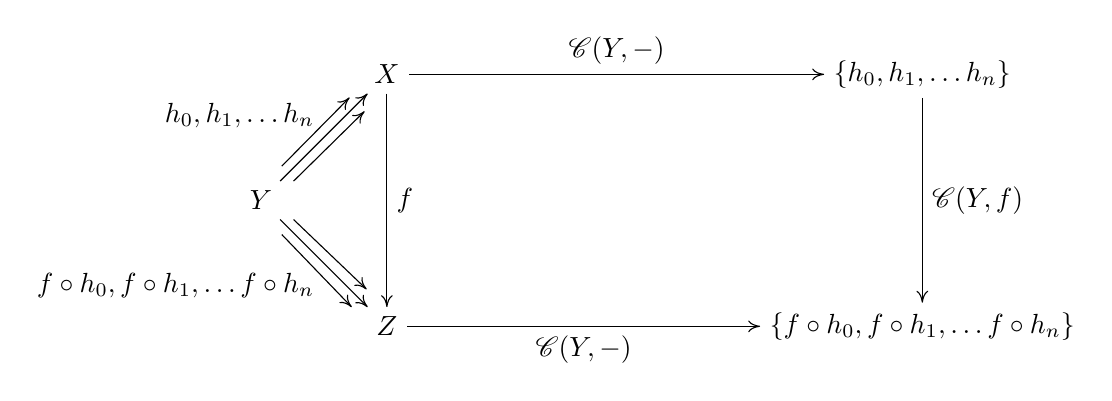
\begin{tikzpicture}
            \node(X) at ( 0 , 0 ) {$X$};
            \node(Y) at ( -16mm , -16mm ) {$Y$};
            \node(Z) at ( 0 , -32mm ) {$Z$};
            \node(homYX) at (68mm , 0 ) {$\{ h_0, h_1, \dots h_n \}$};
            \node(homYZ) at (68mm , -32mm ) {$\{ f \circ h_0, f \circ h_1, \dots f \circ h_n \}$};
            \draw [morphism] (X) -- (Z) node [midway, right] {$f$};
            \draw [morphism] (X) -- (homYX) node [midway, above] {$\mathscr{C}(Y,-)$};
            \draw [morphism] (Z) -- (homYZ) node [midway, below] {$\mathscr{C}(Y,-)$};
            \draw [morphism] (Y) -- (X) node [midway, above left] {$h_0, h_1,\dots h_n$};
            \draw [morphism] ($(Y.north east)+(0,1.9mm)$) -- ($(X.south west)+(-1.9mm,-0.5mm)$);
            \draw [morphism] ($(Y.north east)+(1.5mm,0)$) -- ($(X.south west)+(0mm,-2.25mm)$);

            \draw [morphism] (Y) -- (Z) node [midway, below left] {$f\circ h_0, f\circ h_1,\dots f\circ h_n$};
            \draw [morphism] ($(Y.south east)+(0,-1.9mm)$) -- ($(Z.north west)+(-1.9mm,0mm)$);
            \draw [morphism] ($(Y.south east)+(1.5mm,0mm)$) -- ($(Z.north west)+(0mm,2.25mm)$);
            \draw [morphism] (homYX) -- (homYZ) node [midway, right] {$\mathscr{C}(Y,f)$};
        \end{tikzpicture}
    \end{center}

    \noindent Now suppose we set $Z = X$ and $f = \mathbf{id}_X$:

    \begin{center}
        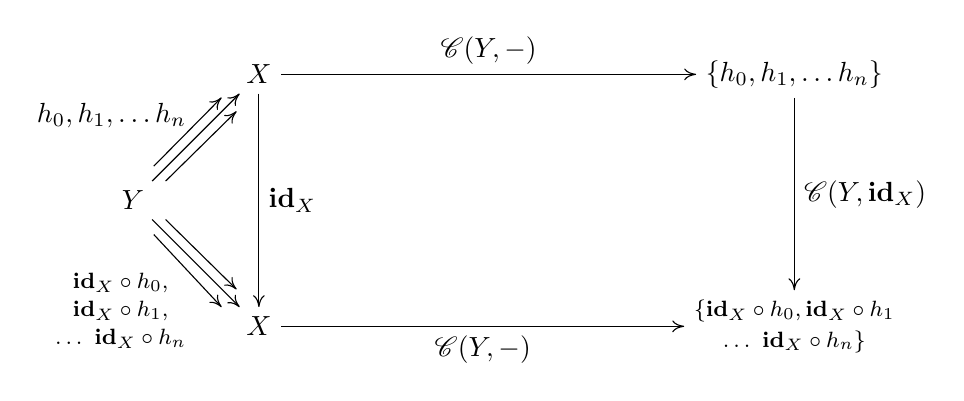
\begin{tikzpicture}
            \node(X) at ( 0 , 0 ) {$X$};
            \node(Y) at ( -16mm , -16mm ) {$Y$};
            \node(Z) at ( 0 , -32mm ) {$X$};
            \node(homYX) at (68mm , 0 ) {$\{ h_0, h_1, \dots h_n \}$};
            \node(homYX2) at (68mm , -32mm ) {
                \footnotesize
                \shortstack{
                    $\{ \mathbf{id}_X \circ h_0, \mathbf{id}_X \circ h_1$ \\  
                    $\dots\ \mathbf{id}_X \circ h_n \}$
                }
            };
            \draw [morphism] (X) -- (Z) node [midway, right] {$\mathbf{id}_X$};
            \draw [morphism] (X) -- (homYX) node [midway, above] {$\mathscr{C}(Y,-)$};
            \draw [morphism] (Z) -- (homYX2) node [midway, below] {$\mathscr{C}(Y,-)$};
            \draw [morphism] (Y) -- (X) node [midway, above left] {$h_0, h_1,\dots h_n$};
            \draw [morphism] ($(Y.north east)+(0,1.9mm)$) -- ($(X.south west)+(-1.9mm,-0.5mm)$);
            \draw [morphism] ($(Y.north east)+(1.5mm,0)$) -- ($(X.south west)+(0mm,-2.25mm)$);

            \draw [morphism] (Y) -- (Z) node [midway, below left] { 
                \footnotesize
                \shortstack{ 
                    $\mathbf{id}_X\circ h_0,$ \\ 
                    $\mathbf{id}_X\circ h_1,$ \\ 
                    $\dots\ \mathbf{id}_X\circ h_n$
                }
            };
            \draw [morphism] ($(Y.south east)+(0,-1.9mm)$) -- ($(Z.north west)+(-1.9mm,0mm)$);
            \draw [morphism] ($(Y.south east)+(1.5mm,0mm)$) -- ($(Z.north west)+(0mm,2.25mm)$);
            \draw [morphism] (homYX) -- (homYX2) node [midway, right] {$\mathscr{C}(Y,\mathbf{id}_X)$};
        \end{tikzpicture}
    \end{center}

    \noindent We now see that for all $Y \xrightarrow{\ h \ } X$ the function $\mathscr{C}(Y,\mathbf
    {id}_X)$ maps $h$ to $\mathbf{id}_X \circ h$. By the definition of the identity morphism, 
    $\mathbf{id}_X \circ h \equiv h$. Therefore, $\mathscr{C}(Y,\mathbf{id}_X)$ is precisely the 
    identity function on the homset $\mathscr{C}(Y,X)$. A similar argument may be constructed for 
    the contravariant case.

    \begin{question}
        Show that \texttt{Maybe} is not representable.
    \end{question}
    We can make an argument based on cardinality. Any isomorphism between sets must be bijective, 
    and in order to form a bijection between two sets, they must have the same 
    cardinality. For any type \texttt{T} with cardinality $t$, the type \texttt{Maybe<T>} will have 
    cardinality $t+1$. Given any candidate representing type \texttt{R}, the function type \texttt
    {R $\to$ T} will have cardinality $t^r$. This means that we must find some $r$ such that $t^r = 
    t+1$. Rearranging, we find that $r = \log_t (t+1)$. For $t=1$, we find $r$ is undefined, for 
    $t=2$, $r = 1.5849...$---we will struggle to find a type with such cardinality! The function 
    tends toward 1 as $t$ approaches infinity, so we have no hope of finding an integer-valued 
    result.

    \pagebreak

    \begin{question}
        Is the \texttt{Reader} functor representable?
    \end{question}
    Yes, since \texttt{Reader} maps two types \texttt{A} and \texttt{B} onto their function type 
    \texttt{A $\to$ B}, it is trivially representable.

    \begin{question}
        Using \texttt{Stream} representation, memoize a function that squares its argument.
    \end{question}
    (See accompanying \texttt{F\#} script.)

    \begin{question}
        Show that \texttt{tabulate} and \texttt{index} for Stream are indeed the inverse of each 
        other. (Hint: use induction.)
    \end{question}

    I don't think there's any way to do this other than the solution written here:\\
    http://danshiebler.com/2018-11-10-category-solutions/

    \begin{question}
        The functor: \texttt{Pair a = Pair a a} is representable. Can you guess the type that 
        represents it? Implement tabulate and index.
    \end{question}

    We can make another cardinality argument. Given a type \texttt{T} with cardinality $t$, The 
    type \texttt{Pair<T>}, has cardinality $t \times t$. This means that the function \texttt{R 
    $\to$ T} must also have cardinality $t \times t$. Which means we must find a type with 
    cardinality $r$ such that $t^r = t \times t$. This is plainly 2, so we can easily choose \texttt
    {Bool} for \texttt{R}; however, we may wish to choose something with more descriptive values 
    (such as \texttt{fst} and \texttt{snd}, \texttt{car} and \texttt{cdr}, or \texttt{left} and 
    \texttt{right}), as any type of cardinality 2 will do the trick. Implementation is provided in
    the accompanying script.


\end{document}